\documentclass[../main.tex]{subfiles}
\begin{document}


For this paper, I will calculate the metrics Dey et al. proposed for MDS corpora to a dataset myself.
The corpus was selected on the following criteria:

\begin{itemize}
    \item must be MDS corpus - the metrics were specifically designed for MDS corpora, and some, like Inter Document Similarity, only make sense in this context.
    \item must not already have been analyzed with these metrics, either in the original paper or by its creators
    \item should be somewhat recent
    \item dataset must be publicly available
\end{itemize}

This last criterion was actually the most constraining. I opted for the "Wikipedia Current Events Portal" (WCEP) dataset, proposed in 2020. \cite{WCEP-gholipour-ghalandari-etal-2020-large}
It meets all of the conditions mentioned above, as it was published in 2020, was designed explicitly for MDS, does not include the metrics from the original paper (which was published after WCEP) and the authors provide a public download link to the entire dataset on their GitHub.\cite{WCEP-Github-complementizer_2022}


Although the original papers authors state that they "develop an interactive web portal for imminent corpora to be uploaded and evaluated based
on [their] proposed metrics", I was unable to find any link or other kind of reference to this.
The paper does, however, include a link to the source code for their analysis on GitHub, which although lacking documentation, served as the starting point for the following analysis of WCEP.

For this paper I have forked the repository and updated the code for the corpus metrics to work with the WCEP dataset.
I have also added documentation on how to use the code and which format the data is expected to have, which is missing in the original version.


The WCEP dataset is split into 3 parts, a vary large training set and the test and validation sets, which each make up about 10 percent of the total amount.
For this evaluation, I treated them as separate datasets, so that I could determine if they are homogenous.

For this task, I modified the source code provided by the authors slightly, in order to make this analysis possible. The version of the code used for this analysis is available on my Github \footnote{Repository: \url{https://github.com/layaxx/summarization_bias}}.

\begin{figure}
    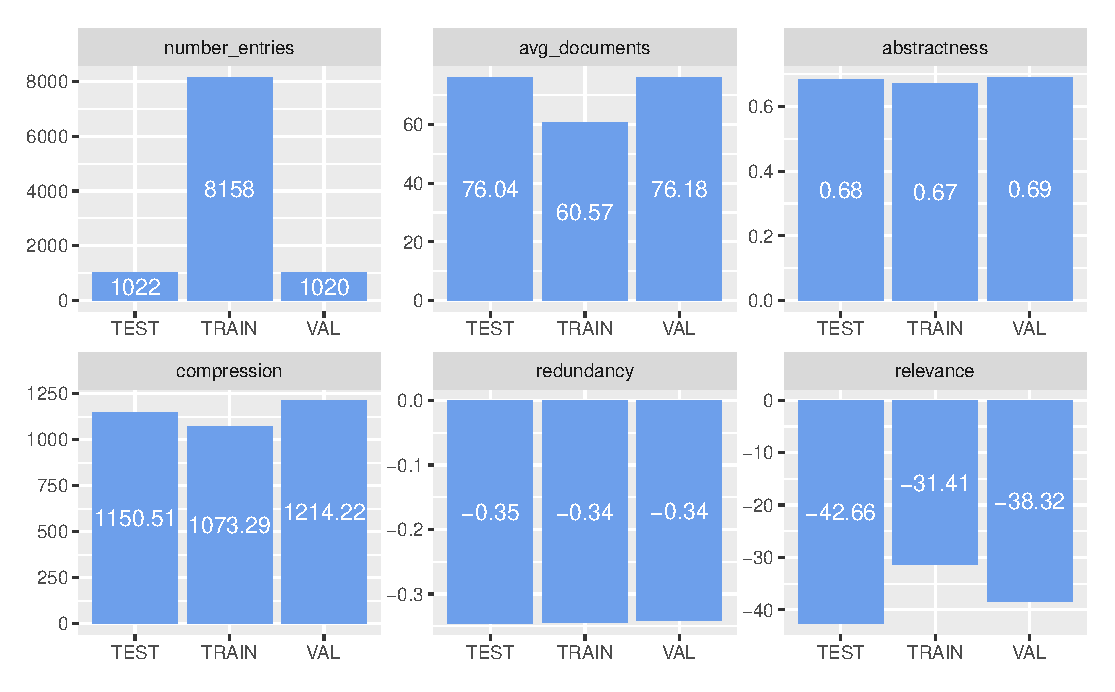
\includegraphics[width=\textwidth]{figures/analysis.eps}
    \caption{Overview over the benchmark results calculated from the WCEP corpus. Every metric is reported for each of the testing, training and validation subsets of WCEP.} \label{fig:analysis}
\end{figure}

The results can be seen in \ref{fig:analysis}. "number\_entries" denotes the number of topics in each set, consisting of one reference summary and a set of documents.
The average number of documents per set is shown as "avg\_documents". "abstractness", "compression", and "redundancy" are the same as described in the original paper.
With the "relevance" metric, I am unsure whether this is identical to IDS or just a precursor to its calculation.

While the other metrics were calculated for the complete set, due to high computational demands redundancy and relevance have been calculated on a random sample consisting of 100 topics for each of the three subsets.

I have not been able to measure the Layout Bias and the Pyramid Scores, as it is unclear to me what format the original authors code expect for the input to calculation.

Apart from obvious differences in size, the subsets of WCEP seem pretty homogenous after analysis.
Notable differences are, however, visible on the relevance and average documents per topic metrics.
The training set contains, on average, 15.47 (20.34\%) less documents per topic compared with the test set and 15.61 (20.49\%) less than the validation set.
The relevancy of the training set is also notably closer to 0 compared with the other subsets.

% TODO: plot distribution of number of articles / article length?

\begin{figure}
    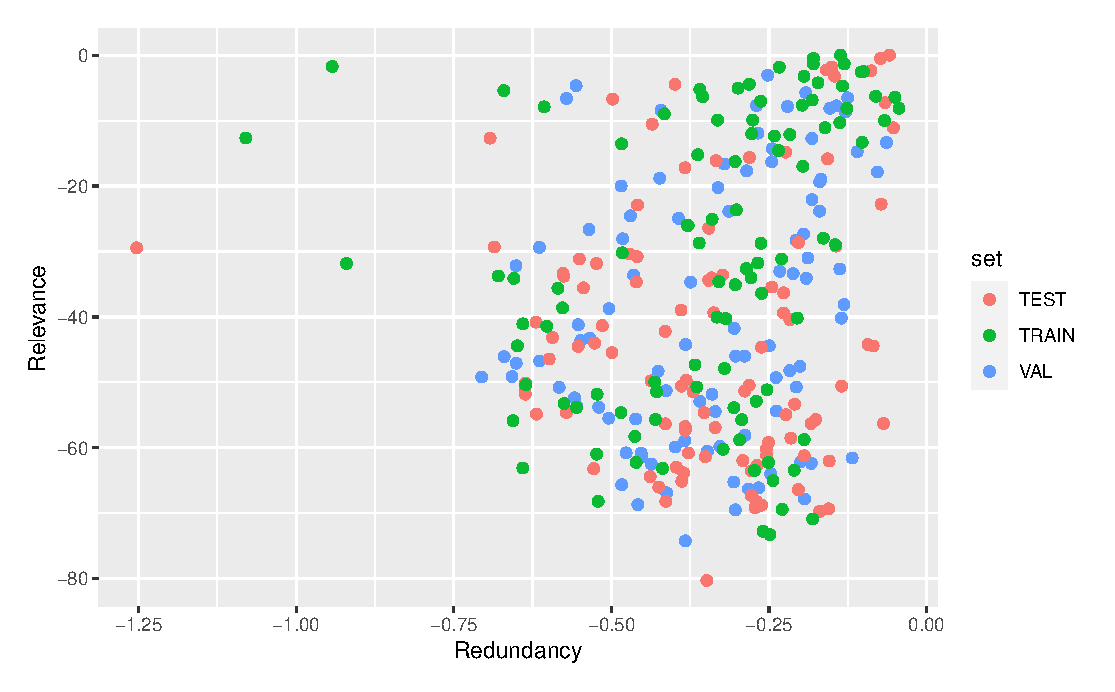
\includegraphics[width=\textwidth]{figures/analysis-2.eps}
    \caption{Scatter plot of Relevance and Redundancy shows no obvious difference between the subsets.} \label{fig:analysis-2}
\end{figure}


\begin{figure}
    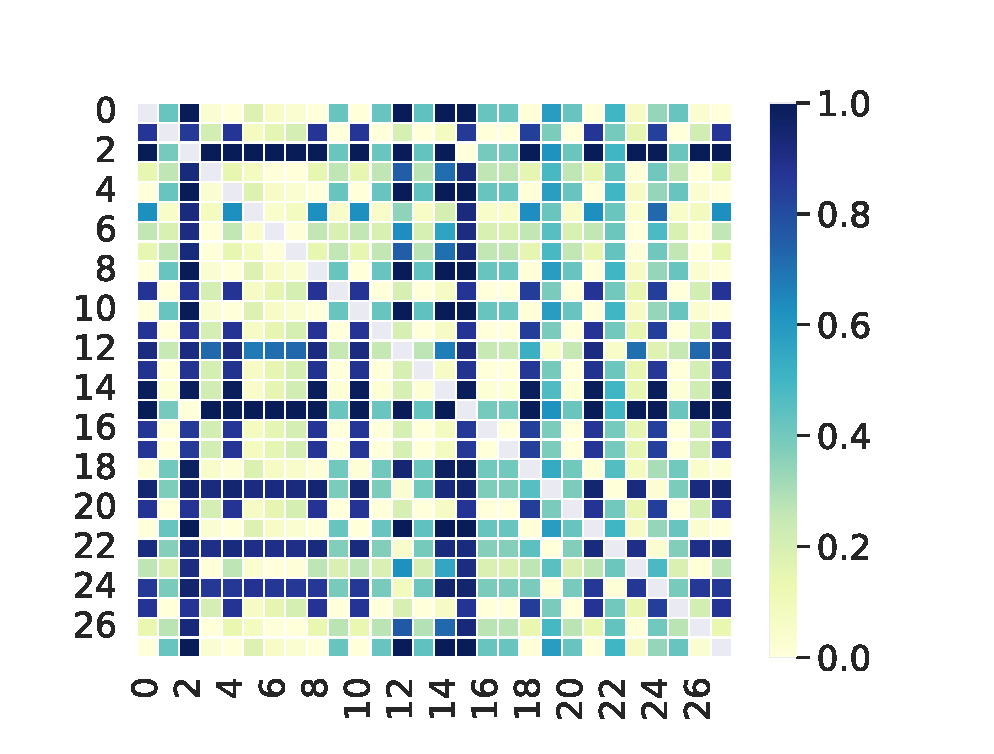
\includegraphics[width=.49\textwidth]{figures/test70168.eps}
    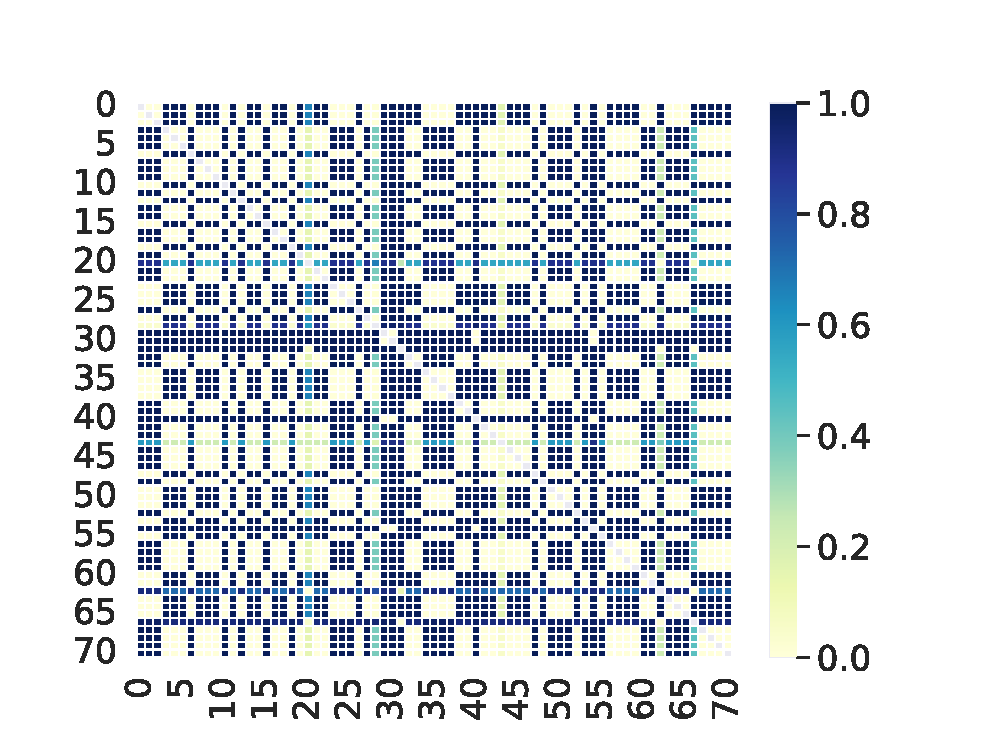
\includegraphics[width=.49\textwidth]{figures/train62667.eps}
    \caption{Example plot of IDS for topic 70168 from the test subset and topic 62667 from the training set.} \label{fig:analysis-ids-test}
\end{figure}

\end{document}